\section{Numerical examples}
\label{section: Chapter4/examples}

In this Section, a two example problems computed with the aforementioned method are presented. These examples illustrate the main capabilities of the approach, but also serve to demonstrate some of the limitations. They all consist of hydrulic fracture propagation in a poroelastic medium involving different fracture configurations that are relevant to practical fracking applications. The main goal is to ensure that the proposed algorithm supports these two representative scenarios and that it can be used to simulate real world fracking treatments whenever the assumption of planar growth is adequate. 

Importantly, a true verification procedure is not performed here. For example, mesh convergence studies and comparisons with well-known solutions are yet to be performed for these 3D problems as we did in Chapter \ref{section: Chapter3}. These require a few enhancements in the solver technology that are currently under development. First, due to the high discrepancy between the scales of degrees of freedom (matrix displacements, fracture apertures and pressures), general purpose linear solvers struggle to converge when the meshes are refined past a certain point. Because of that, special preconditioners that take into account the block structure of the system are being developed. Second, analytical solutions for poroelastic problems are scarce, so, a common verification procedure consists in solving them with vanishing small permeability coefficients to verify convergence towards the impermeable case, which does have a closed-form solution. However, as the permeability decreses, the poromechanics problem starts to display spurious pressure oscillations unless LBB-stable elements \cite{arnold1984stable} or a stabilized formulations, such as \cite{white2008stabilized} are used. These enhancements in the solver infrastructure are left for future work.

For the two problems in this Section, the material properties used are listed in Table \ref{material properties ch4}. 

\begin{table}[h]
  \centering
  \caption{Material properties for planar fracture problems.}
  \begin{tabular}[t]{lcc}
  \hline
  &Value &Unit \\
  \hline
  Young's modulus ($E$)&16.0&GPa\\
  Poisson's ratio ($\nu$)&0.18&--\\
  Fluid viscosity ($\mu$)&1.0$\times10^{-12}$&$\text{GPa . s}$\\
  Fluid bulk modulus ($K_f$)&1.0$\times10^{10}$&$\text{GPa}$\\
  Critical energy release rate ($G_c$)&2.5&$\text{N/m}$\\
  Biot coefficient ($\alpha$)&1.0&$\text{ - }$\\
  Rock permeability ($\kappa_0$)&1.0$\times 10^{-13}$&$\text{m}^2$\\
  Initial porosity ($\phi_0$)&0.2&$\text{-}$\\
  \hline
  \end{tabular}
  \label{material properties ch4}
\end{table}%

\subsection{Two parallel circular fractures under fluid injection}

In the first problem, a pair of parallel penny-shaped fractures is stimulated with the injection of a viscous fluid. This configuration is representative of a very common scenario in real-world fracking treatments where, in general, there are multiple clusters with several parallel fractures in each. Their simultaneous stimulation can lead to all fractures growing simultaneously or to situations in which only a few show substantial propagation while the others arrest early in the process. These scenarios can lead to very different well behaviors.   

Depending on the distance between the fractures, there may also be non-planar growth, with fractures propagating away from each other, forming a cup shaped geometry. This is a consequence of the interaction between the stress fields in the vicinity of the multiple fractures fronts. This interaction is often called stress shadow effect. In this numerical example shown here, the initial fractures are placed far from each other to prevent this non-planar behavior. The far-field boundary conditions are assumed to be homogenous for pressures and displacements. Figure \ref{fig:parallel_schematic} illustrates the geometry. The dimensions are described in Table \ref{parallel_measures}.

As for the discretization, the coarser global mesh consists of a structured grid that is refined near the fracture planes, with an element size of around 0.075m in the width direction and 0.15m in the other directions. The local mesh is 5 times smaller and the regularization length used in the phase-field subproblem is 0.05m. Importantly, the local domain consists of all local elements within a distance of 1m to the fracture front. Since the fractures are penny shaped, this local domain will have the shape of a torus. As for the time-step, it is uniformly set to 0.01s.

Due to the uniform boundary conditions and homogenous material properties, the fractures are expected to grow radially, preserving their circular shape. This feature is confirmed in the simulated results shown in Figure \ref{fig:parallel_snapshots}. In these snapshots, the right-side of the domain shows the pressure field computed in the global domain whereas the left side shows the discrete crack geometry, colored in gray scale indicating the aperture field. This figure also shows the subdomain around the crack front, colored by the damage field.

The aperture and pressure at the injection sources are important quantities of interest in this type of problem and their simulated time series are shown in Figure \ref{fig:parallel_fracs_charts}. Due to the symmetry, both fractures have the same pressure and aperture results. The reference values used to make the curves nondimensional are listed in Table \ref{parallel_refs}.

\begin{table}[ht]
  \centering
  \caption{Domain dimensions}
  \begin{tabular}[t]{lccccccc}
  \hline
  &$d_1$&$d_2$&$d_3$&$L_x$&$L_y$&$L_z$&$r$\\  
  \hline
  Value (m) & 4.0 & 8.0 & 4.0 & 16.0 & 5.0 & 5.0 & 1.3\\
  \hline
  \end{tabular}
  \label{parallel_measures}
\end{table}%

\begin{table}[ht]
  \centering
  \caption{Reference values used in the time series plots.}
  \begin{tabular}[t]{lcc}
  \hline
  &Value &Unit \\
  \hline
  $p_{ref}$&$320$&MPa\\
  $w_{ref}$&$4.0\times10^{-4}$&m\\
  $t_{ref}$&$10$&$\text{s}$\\
  \hline
  \end{tabular}
  \label{parallel_refs}
\end{table}%

\begin{figure}[ht]
  \centering
  \begin{tikzpicture}
      \node {\pgfimage[interpolate=false,width=0.8\textwidth]{Chapter4/figures/3D/parallel_schematic.png}};
      \draw (-0.11\textwidth,0.185\textwidth) node {\large$r$};
      \draw (0.3\textwidth,0.12\textwidth) node {\large$L_x$};
      \draw (0.1\textwidth,-0.31\textwidth) node {\large$L_y$};
      \draw (0.42\textwidth,-0.15\textwidth) node {\large$L_z$};
      \draw (-0.05\textwidth,0.3\textwidth) node {\large$d_1$};
      \draw (0.02\textwidth,0.23\textwidth) node {\large$d_2$};
      \draw (0.09\textwidth,0.15\textwidth) node {\large$d_3$};
  \end{tikzpicture}
  \caption{Schematic of the problem geometry.}
  \label{fig:parallel_schematic}
\end{figure}


\begin{figure}[h]
  \noindent% This file was created with tikzplotlib v0.10.1.
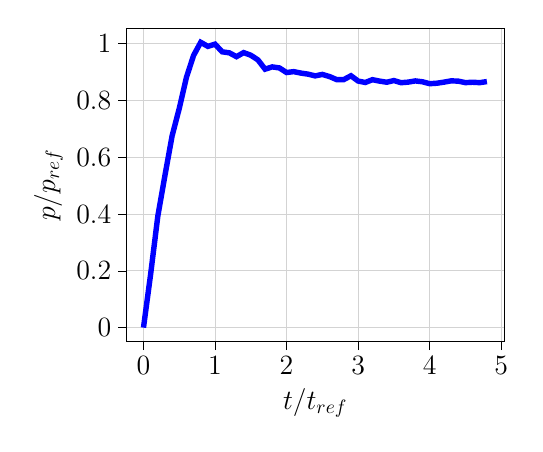
\begin{tikzpicture}[scale=0.7, font=\Large]

\definecolor{lightgray}{RGB}{211,211,211}

\begin{axis}[
tick align=outside,
tick pos=left,
x grid style={lightgray},
xlabel={\(\displaystyle t/t_{ref}\)},
xmajorgrids,
xmin=-0.24, xmax=5.04,
xtick style={color=black},
y grid style={lightgray},
ylabel={\(\displaystyle p/p_{ref}\)},
ymajorgrids,
ymin=-0.0502281761912294, ymax=1.05479170001582,
ytick style={color=black}
]
\addplot [line width=2.8pt, blue]
table {%
0 0
0.1 0.188445766752718
0.2 0.391947508110223
0.3 0.535895204930158
0.4 0.675176372415468
0.5 0.771710290038251
0.6 0.880899367078848
0.7 0.958412412909037
0.8 1.00456352382459
0.9 0.990324948221893
1 0.998054606057314
1.1 0.971102817197564
1.2 0.967556258546069
1.3 0.954084839144053
1.4 0.968359167181806
1.5 0.959116405852193
1.6 0.942617944583139
1.7 0.910026091662552
1.8 0.918049400613525
1.9 0.914348525898006
2 0.898192078875057
2.1 0.901362856789026
2.2 0.896214438996315
2.3 0.892511564645737
2.4 0.886358846124087
2.5 0.891502924804546
2.6 0.884023936770732
2.7 0.873345919605794
2.8 0.873412882862689
2.9 0.886829564180904
3 0.868198311002277
3.1 0.863129333961807
3.2 0.873000347785484
3.3 0.867964509851173
3.4 0.864042793812506
3.5 0.869939165930708
3.6 0.862387111210862
3.7 0.864402846886308
3.8 0.868605632794512
3.9 0.865597652226709
4 0.8589197342603
4.1 0.860522133055493
4.2 0.864358319941601
4.3 0.868875836425173
4.4 0.867843224744737
4.5 0.862641238764823
4.6 0.863963070087864
4.7 0.862565672752955
4.8 0.866328855022948
};
\end{axis}

\end{tikzpicture}

  \hspace{0.5cm}
  % This file was created with tikzplotlib v0.10.1.
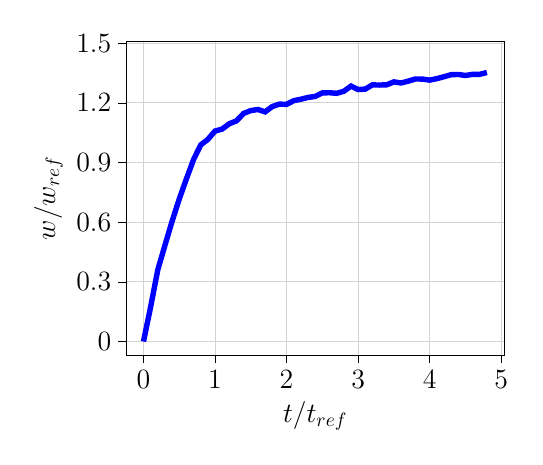
\begin{tikzpicture}[scale=0.7, font=\Large]

\definecolor{lightgray}{RGB}{211,211,211}

\begin{axis}[
tick align=outside,
tick pos=left,
x grid style={lightgray},
xlabel={\(\displaystyle t/t_{ref}\)},
xmajorgrids,
xmin=-0.24, xmax=5.04,
xtick style={color=black},
y grid style={lightgray},
ytick distance=0.3,
ylabel={\(\displaystyle w/w_{ref}\)},
ymajorgrids,
ymin=-0.0676150128188689, ymax=1.51,
ytick style={color=black}
]
\addplot [line width=2.8pt, blue]
table {%
0 0
0.1 0.174099460537345
0.2 0.36037093622801
0.3 0.483736302329922
0.4 0.604657400483929
0.5 0.71627362525909
0.6 0.817741763252065
0.7 0.914673087058184
0.8 0.988043835003288
0.9 1.01615749619579
1 1.05781999647227
1.1 1.06795558571426
1.2 1.09487671410362
1.3 1.10903211791217
1.4 1.14665606861212
1.5 1.16093104459679
1.6 1.16625499737314
1.7 1.15430886393875
1.8 1.18121700420342
1.9 1.19330912726223
2 1.19206895215774
2.1 1.21057291458408
2.2 1.21798236109138
2.3 1.22691783387849
2.4 1.23188777939765
2.5 1.24970648339836
2.6 1.25053556512246
2.7 1.24766343959738
2.8 1.2578584515492
2.9 1.28381515930564
3 1.26659534216305
3.1 1.26894556444263
3.2 1.29005564497642
3.3 1.28918001813621
3.4 1.29050708947248
3.5 1.30520754884353
3.6 1.29951568143079
3.7 1.30872862561227
3.8 1.31974418932991
3.9 1.31922767023963
4 1.31398053120865
4.1 1.32143831069796
4.2 1.33095372857038
4.3 1.34126355648886
4.4 1.34234868328863
4.5 1.33716954069027
4.6 1.34310704227726
4.7 1.34310814299716
4.8 1.35230025637738
};
\end{axis}

\end{tikzpicture}

  \caption{Two quantities of interest for the parallel fracture problem. On the left, the time series of the pressure at the injection point, on the right, the fracture aperture. Both plots show results scaled by reference values, calculated at the onset of propagation.}  
  \label{fig:parallel_fracs_charts}
\end{figure}


\begin{figure}[h]
\begin{subfigure}{.45\textwidth}
  \centering
  \includegraphics[width=\linewidth]{Chapter4/figures/3D/new_t_0.png}
  \caption{}
  \label{fig:parallel_t_0}
\end{subfigure}%
\hspace{1cm}
\begin{subfigure}{.45\textwidth}
  \centering
  \includegraphics[width=\linewidth]{Chapter4/figures/3D/new_t_30.png}
  \caption{}
  \label{fig:parallel_t_1}
\end{subfigure}%

\begin{subfigure}{.45\textwidth}
  \centering
  \includegraphics[width=\linewidth]{Chapter4/figures/3D/new_t_60.png}
  \caption{}
  \label{fig:parallel_t_2}
\end{subfigure}
\hspace{0.85cm}
\begin{subfigure}{.45\textwidth}
  \centering
  \includegraphics[width=\linewidth]{Chapter4/figures/3D/new_t_90.png}
  \caption{}
  \label{fig:parallel_t_3}
\end{subfigure}
  \caption{Snapshots of the simulated propagation. The left side of the figures shows the discrete fracture colored in grayscale according to the aperture and the subdomain colored according the damage value. The right side shows the pressure field in the global domain. (a) Snapshot $t/t_{ref} = 0$; (b) $t/t_{ref} = 1.5$; (c) $t/t_{ref} = 3$; and (d) $t/t_{ref} = 4.5$. } 
  \label{fig:parallel_snapshots}
\end{figure}

\FloatBarrier

\subsection{Merging two circular fractures}

The second problem deals with the case of in-plane fracture merging. In general, fracture merging is one of the most difficult behaviors to simulate with discrete fracture approaches. That is due to the interaction between the stress fields of two fracture fronts, which makes most attempts to extract a stress intensity factor innacurate. In practice, these situation may happen when fracking wells are drilled parallel to each other. 

For problems involving crack merging, the phase-field approach becomes handy, allowing for the computation of crack advances through the solution of PDEs that are independent of the fracture topology.
The multi-resolution approach explore this advantage, keeping a phase-field description around the fracture front and removing the limitations of discrete methods.

Since this problem deals with in-plane merging, getting the discrete fracture planes from the phase-field values is straightforward. However, it is important to mention that this can be a challenge in the case of non-planar merging.

The problem under consideration consists of two parallel fractures, initally of circular shape, embedded in a poroelastic matrix. Both are injected with a viscous fluid and propagate radially, eventually merging. An schematic of the geometry is shown in Figure \ref{fig:merging_schematic}, with the dimensions listed in Table \ref{merging_measures}. As in the previous problem, the far-field boundary conditions are assumed to be homogenous for pressures and displacements. 

As for the discretization, the coarser global mesh consists of a structured grid that is refined near the fracture planes, with an element size of around 0.095m in the width direction and 0.15m in the other directions. The local mesh is 5 times smaller and the regularization length used in the phase-field subproblem is 0.05m. Importantly, the local domain consists of all local elements within a distance of 1m to the fracture front. Initally, they consist of two separate torus, but they eventually merge as the cracks get closer. As for the time-step, it is uniformly set to 0.01s.

The simulated behavior is depicted in Figure \ref{fig:merge_snapshots}, which shows the expected behavior, which the cracks growing perfectly as circles until they approach each other and merge. After the merge, the most concave part of the crack grows and opens up until the pressure drops enough for the propagation to arrest. While there is not reference solution to compare, at least qualitatively, the results make sense. As for the previous problem, the times series for the aperture and pressure in the injection point are shown in Figure \ref{fig:merging_charts}. The reference values used to make these charts nondimensional are given in Table \ref{merging_refs}.

\begin{table}[ht]
  \centering
  \caption{Domain dimensions}
  \begin{tabular}[t]{lccccccc}
  \hline
  &$d_1$&$d_2$&$d_3$&$L_x$&$L_y$&$L_z$&$r$\\  
  \hline
  Value (m) & 6.5 & 7.0 & 6.5 & 8.0 & 20.0 & 5.0 & 1.5\\
  \hline
  \end{tabular}
  \label{merging_measures}
\end{table}%

\begin{table}[ht]
  \centering
  \caption{Reference values used in the time series plots.}
  \begin{tabular}[t]{lcc}
  \hline
  &Value &Unit \\
  \hline
  $p_{ref}$&0.2&MPa\\
  $w_{ref}$&4.0&m\\
  $t_{ref}$&30&$\text{s}$\\
  \hline
  \end{tabular}
  \label{merging_refs}
\end{table}%

\begin{figure}[ht]
  \centering
  \begin{tikzpicture}
      \node {\pgfimage[interpolate=false,width=.8\textwidth]{Chapter4/figures/merging/merging_schematic.png}};
      \draw (0.0\textwidth,0.07\textwidth) node {\large$r$};
      \draw (0.37\textwidth,0.12\textwidth) node {\large$L_x$};
      \draw (0.04\textwidth,-0.25\textwidth) node {\large$L_y$};
      \draw (0.42\textwidth,-0.07\textwidth) node {\large$L_z$};
      \draw (-0.25\textwidth,0.25\textwidth) node {\large$d_1$};
      \draw (-0.03\textwidth,0.25\textwidth) node {\large$d_2$};
      \draw (0.2\textwidth,0.25\textwidth) node {\large$d_3$};
  \end{tikzpicture}
  \caption{Schematic of the geometry for the merging problem.}
  \label{fig:merging_schematic}
\end{figure}


\begin{figure}[h]
\noindent% This file was created with tikzplotlib v0.10.1.
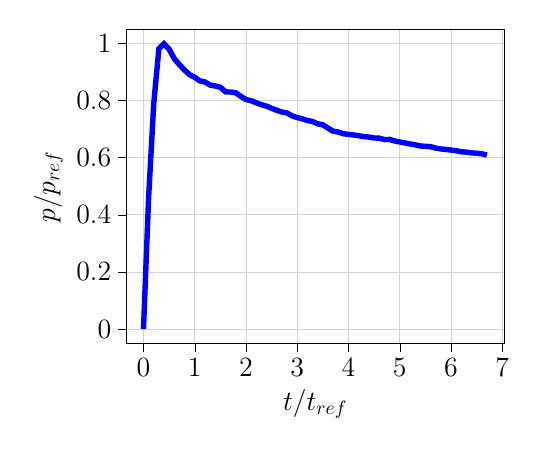
\begin{tikzpicture}[scale=0.7, font=\Large]

\definecolor{lightgray}{RGB}{211,211,211}

\begin{axis}[
tick align=outside,
tick pos=left,
x grid style={lightgray},
xlabel={\(\displaystyle t/t_{ref}\)},
xmajorgrids,
xmin=-0.335, xmax=7.035,
xtick style={color=black},
y grid style={lightgray},
ylabel={\(\displaystyle p/p_{ref}\)},
ymajorgrids,
ymin=-0.0498825329280283, ymax=1.0475331914886,
ytick style={color=black}
]
\addplot [line width=2.8pt, blue]
table {%
0 0
0.1 0.45951217560765
0.2 0.788592266536983
0.3 0.979658043857808
0.4 0.997650658560567
0.5 0.978785067303964
0.6 0.945971757956235
0.7 0.924877167218727
0.8 0.905966129538245
0.9 0.889602759640749
1 0.880357526928354
1.1 0.867671216379265
1.2 0.864233448832077
1.3 0.853114312789821
1.4 0.850108135287821
1.5 0.845620481022948
1.6 0.829505321551291
1.7 0.82892647153026
1.8 0.826514080553166
1.9 0.813655142687903
2 0.802768783688767
2.1 0.798543387344519
2.2 0.791408224631453
2.3 0.784592950157044
2.4 0.779669735090534
2.5 0.771982941261582
2.6 0.764935123584626
2.7 0.759180136109881
2.8 0.755819802453577
2.9 0.745394700232725
3 0.739759343297616
3.1 0.73509236716247
3.2 0.729345702728615
3.3 0.725778734141958
3.4 0.717687645906032
3.5 0.714371573361759
3.6 0.702688940886406
3.7 0.692071117257683
3.8 0.689075788412169
3.9 0.683018346545578
4 0.680940241480926
4.1 0.678761582675207
4.2 0.676155909908243
4.3 0.67303862482668
4.4 0.67141982291266
4.5 0.668213339195578
4.6 0.667744559568312
4.7 0.662721346127251
4.8 0.663129635213632
4.9 0.657892335911165
5 0.654296951897791
5.1 0.650863757765831
5.2 0.647428666367983
5.3 0.644241597549297
5.4 0.640318013987773
5.5 0.638947287170507
5.6 0.638052591816986
5.7 0.632877744620429
5.8 0.629874714646489
5.9 0.62812562862508
6 0.625989632848015
6.1 0.623727478456361
6.2 0.61994558051626
6.3 0.618837276024664
6.4 0.616144894474259
6.5 0.614945973289227
6.6 0.612979236533847
6.7 0.60828213805131
};
\end{axis}

\end{tikzpicture}
\hspace{0.5cm}
\input{Chapter4/figures/tikz/mergingFracAperture.tikz}
\caption{Two quantities of interest for the merging fracture problem. On the left, the time series of the pressure at the injection point, on the right, the fracture aperture. Both plots show results scaled by reference values, calculated at the onset of propagation.}  
\label{fig:merging_charts}
\end{figure}


\begin{figure}[h]
\begin{subfigure}{.45\textwidth}
  \centering
  \includegraphics[width=\linewidth]{Chapter4/figures/merging/merge_t_1(1).png}
  \caption{}
  \label{fig:merge_t_0}
\end{subfigure}%
\hspace{1cm}
\begin{subfigure}{.45\textwidth}
  \centering
  \includegraphics[width=\linewidth]{Chapter4/figures/merging/merge_t_17(1).png}
  \caption{}
  \label{fig:merge_t_1}
\end{subfigure}%

\begin{subfigure}{.45\textwidth}
  \centering
  \includegraphics[width=\linewidth]{Chapter4/figures/merging/merge_t_23(1).png}
  \caption{}
  \label{fig:merge_t_2}
\end{subfigure}
\hspace{0.85cm}
\begin{subfigure}{.45\textwidth}
  \centering
  \includegraphics[width=\linewidth]{Chapter4/figures/merging/merge_t_34(1).png}
  \caption{}
  \label{fig:merge_t_3}
\end{subfigure}

\begin{subfigure}{.45\textwidth}
  \centering
  \includegraphics[width=\linewidth]{Chapter4/figures/merging/merge_t_45(1).png}
  \caption{}
  \label{fig:merge_t_4}
\end{subfigure}
\hspace{0.85cm}
\begin{subfigure}{.45\textwidth}
  \centering
  \includegraphics[width=\linewidth]{Chapter4/figures/merging/merge_t_67(1).png}
  \caption{}
  \label{fig:merge_t_5}
\end{subfigure}
  \caption{Snapshots of the simulated propagation. The discrete fracture is colored in grayscale according to the aperture and the subdomain colored according the damage value. (a) Snapshot $t/t_{ref} = 0$; (b) $t/t_{ref} = 1.3$; (c) $t/t_{ref} = 2.6$; (d) $t/t_{ref} = 3.9$; (e) $t/t_{ref} = 5.2$; and (f) $t/t_{ref} = 6.5$. } 
  \label{fig:merge_snapshots}  
\end{figure}

\FloatBarrier


